\section{Methodology}

\begin{frame}
\begin{center}
     	\huge Methodology
     \end{center}
\end{frame}

\begin{frame}
\frametitle{The Approach}
\begin{figure}
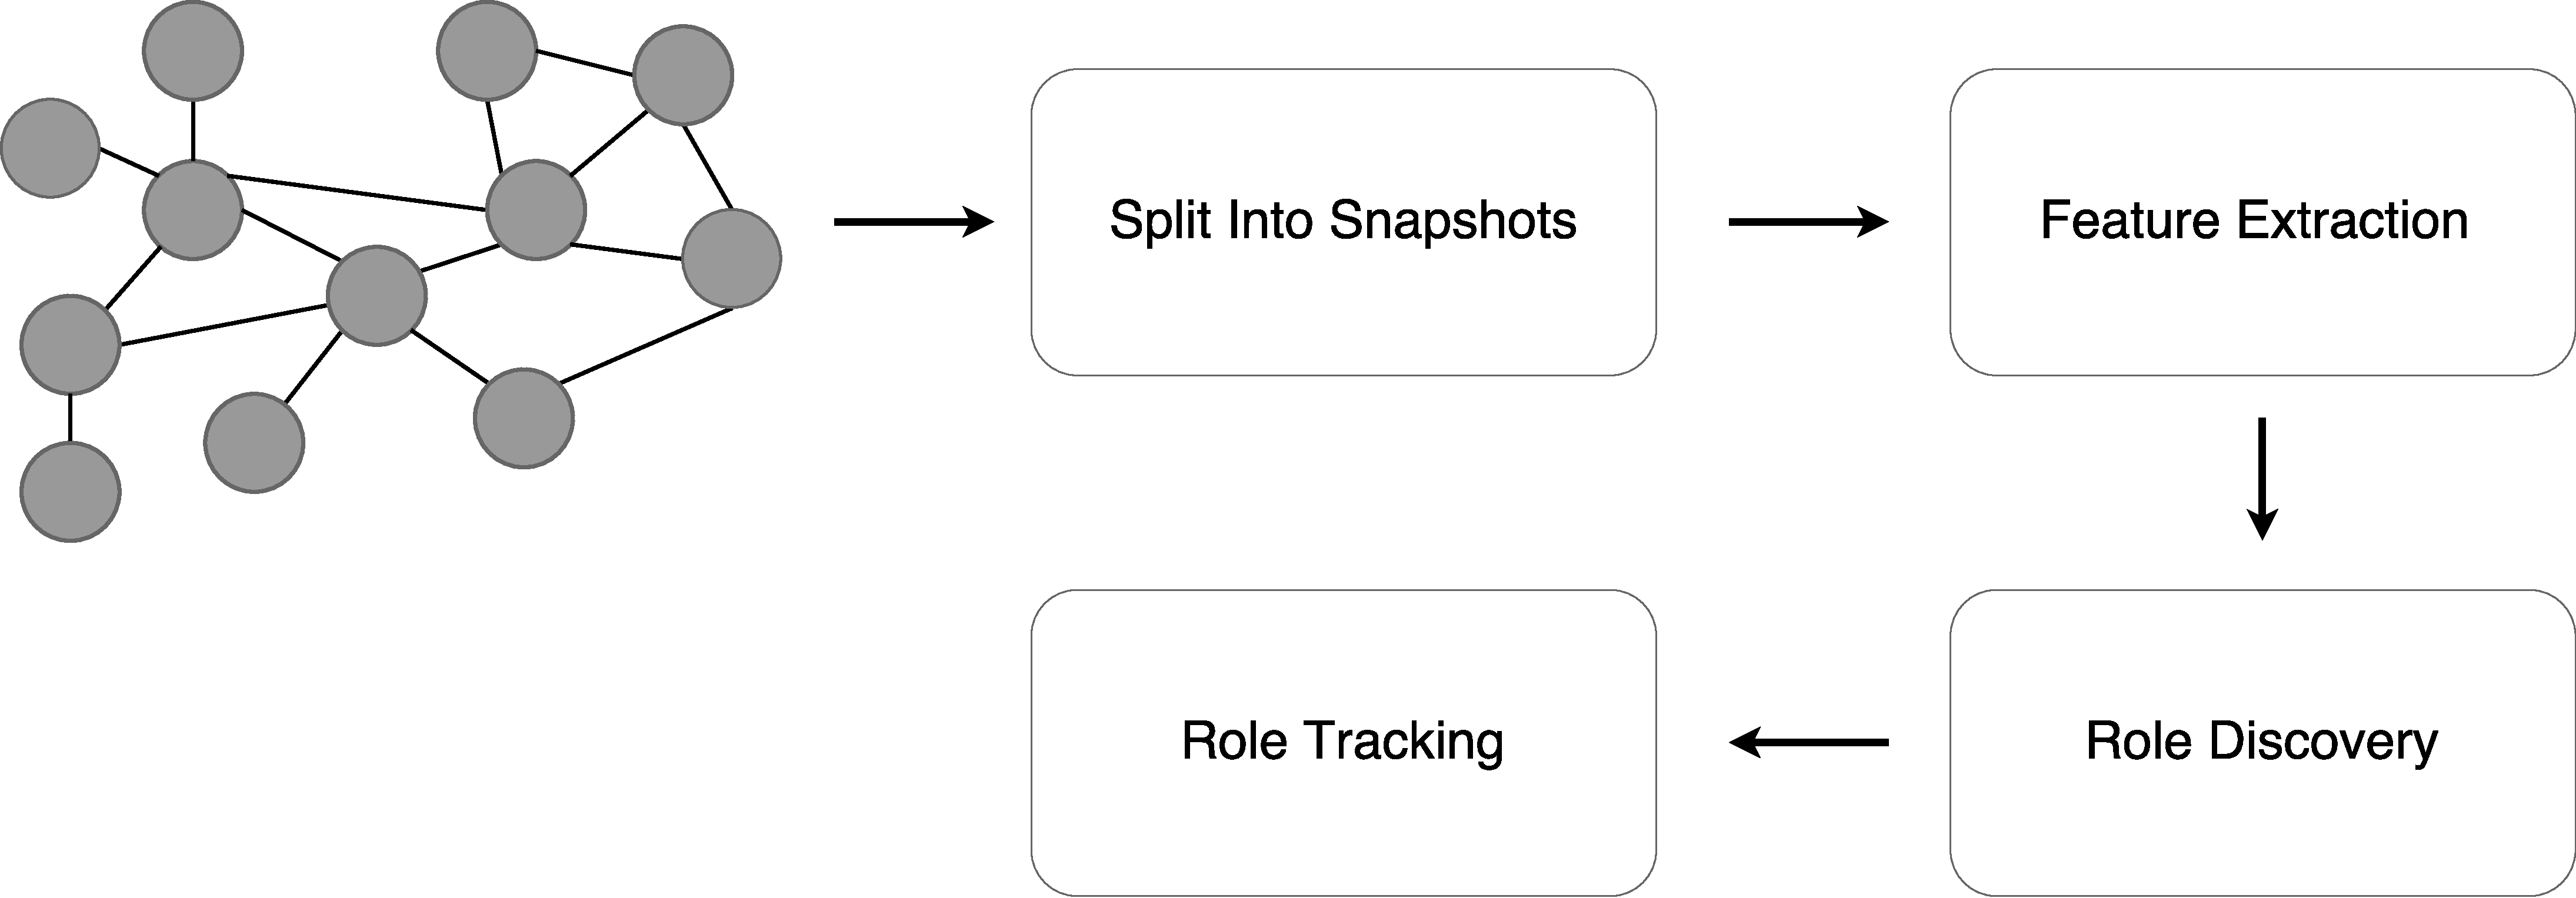
\includegraphics[scale=0.14]{graphics/setup.pdf}
\end{figure}
\note{
feed the data\\
Snapshots:\\
Wanna se the roles lasting over time and networks.\\
Feature extraction:\\
Feature-based approach\\
For each snapshot\\
Role detection:\\
based on the features we wanne find the roles\\
Tracing roles:\\
Making sure the roles are persistent throughout the snapshots 
}
\end{frame}

\begin{frame}
\frametitle{The Data}
\begin{columns}
	\begin{column}{0.45\textwidth}
		Datasets:
			\begin{itemize}
				\item Facebook - Wall posts from one user to another
				\item Scratch - Comments on uploaded programming projects 
			\end{itemize}
		\end{column}
		\begin{column}{0.55\textwidth}
			\begin{figure}
				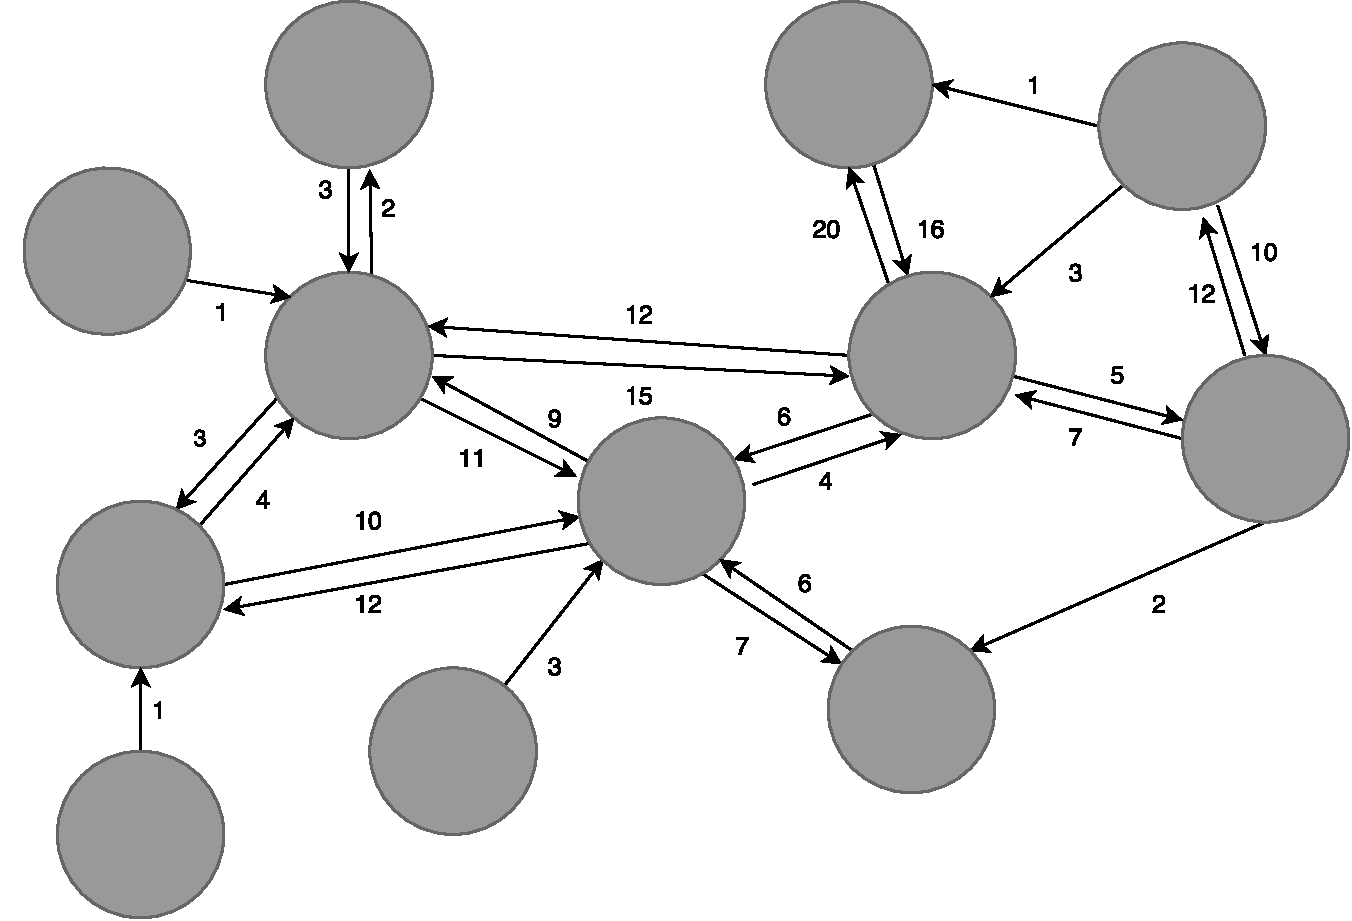
\includegraphics[scale=0.24]{graphics/directed_network.pdf}
			\end{figure}
		\end{column}
	\end{columns}
	\note{
	Facebook post and so one\\
	Scratch comments\\
	The networks are directed and timestamped.\\
	Edges are weighted based on the activity
	}
\end{frame}

\begin{frame}
\frametitle{Snapshots}
The datasets are split into a total of 26 snapshots:
\begin{itemize}
\item 7 from Facebook
\item 19 from Scratch
\end{itemize}
\begin{columns}
	\begin{column}{0.5\textwidth}\centering
			\begin{block} {\small Social Network Graph}
				$D = (N,E)$
			\end{block}
		\end{column}
		\begin{column}{0.5\textwidth}\centering
			\begin{block} {\small Snapshot}
				$S_t = (N_t,E_t)$
			\end{block}
		\end{column}
	\end{columns}
\note{
Non-overlapping\\
Snaps have same length defined as the observation windows $\Omega$\\
$\Omega$ is found by taking the average time between interacting nodes making sure 90\% of the is below $\Omega$
}
\end{frame}

\begin{frame}
\frametitle{Feature Selection}
\begin{columns}
	\begin{column}{0.35\textwidth}
		\begin{itemize}
			\item In-degree 
			\item Out-degree
			\item Weighted in-degree 
			\item Weighted out-degree
		\end{itemize}
	\end{column}
	
	\begin{column}{0.65\textwidth}
		\begin{figure}
			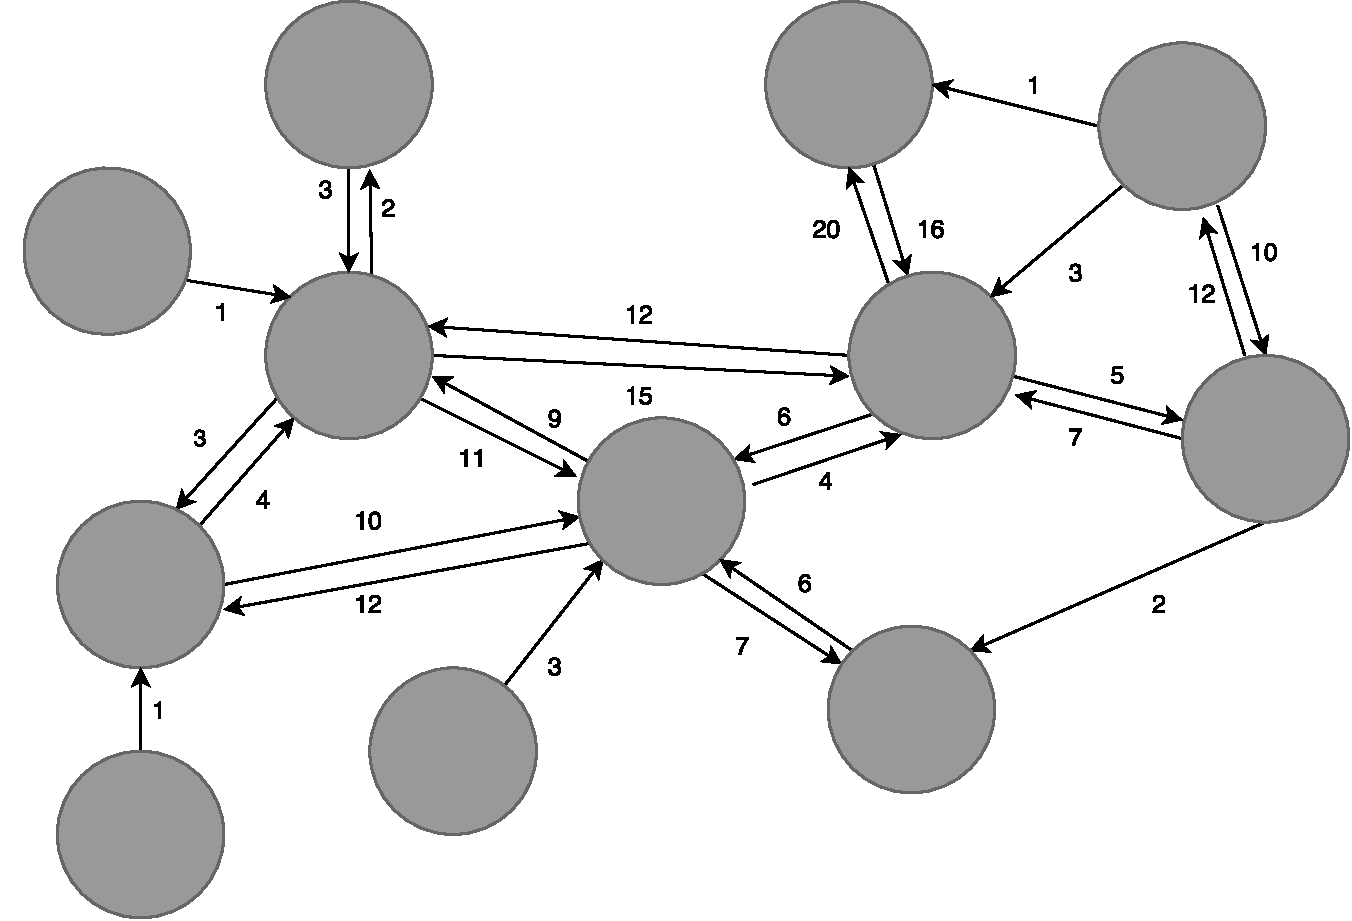
\includegraphics[scale=0.3]{graphics/directed_network.pdf}
		\end{figure}
	\end{column}
\end{columns}
\end{frame}
	
\begin{frame}
\frametitle{Feature Selection}
\textit{Reciprocity} is the rate a user is replayed. The value of this feature is between 1 and 0.
\begin{columns}\centering
\begin{column}{0.5\textwidth}
	\begin{block}{\small Reciprocity}\centering
		$r = \frac{\text{Out-degree}^{<->}}{\text{Out-degree}}$
	\end{block}
\end{column}
\end{columns}
\begin{figure}
	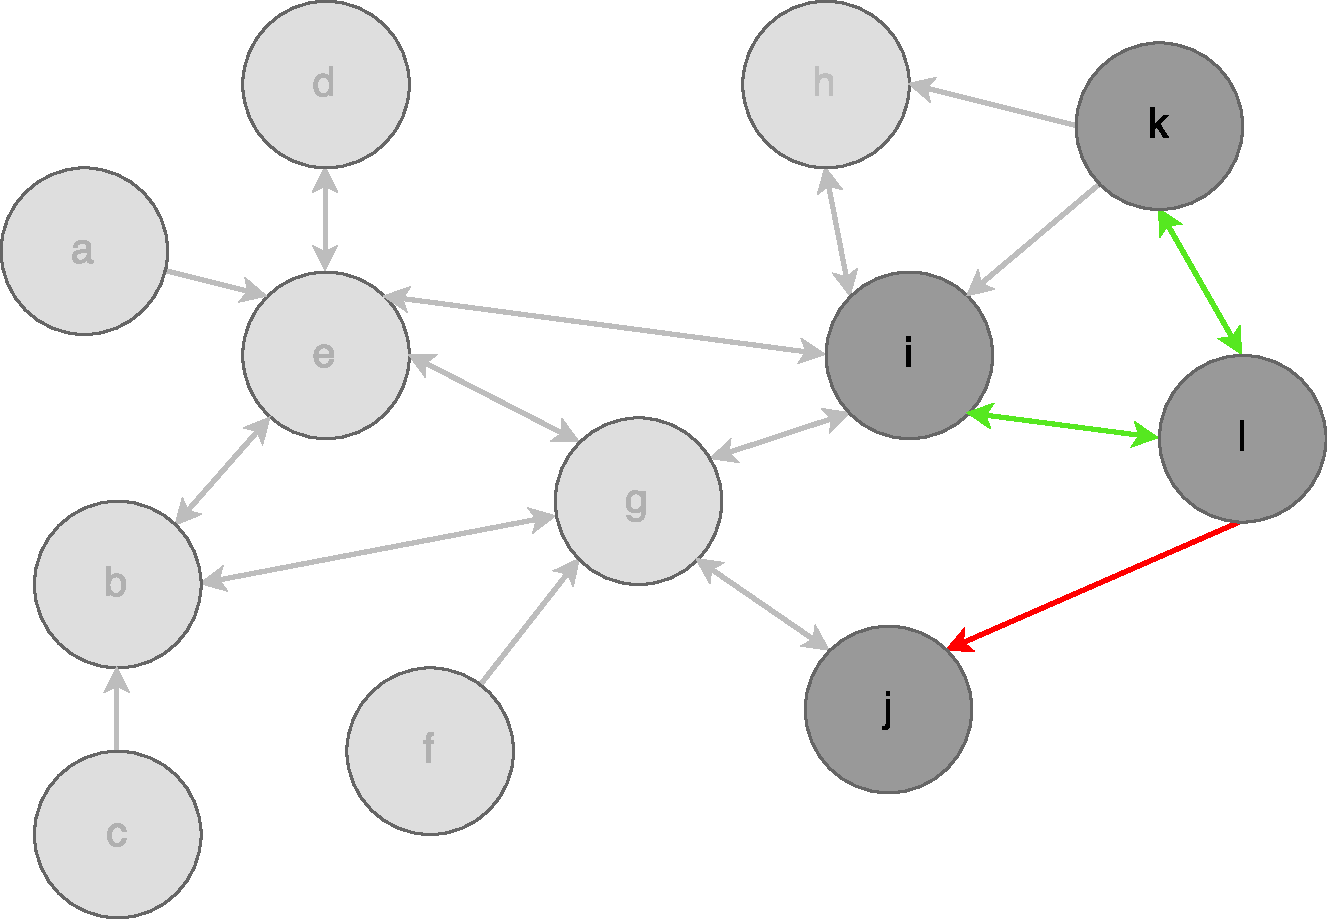
\includegraphics[scale=0.32]{graphics/directed_network_example_reciprocity.pdf}
\end{figure}

\note{
L<-> is the edges going both ways\\
L is all outgoing edges
}
\end{frame}

\begin{frame}
\frametitle{Feature Selection}
The \textit{new activity count} feature is the number of new outgoing edges based on the difference of snapshot $S_t$ and $S_{t-1}$
\begin{columns}\centering
\begin{column}{0.5\textwidth}
	\begin{block}{\small New Activity Count}\centering
		$c = \text{Out-degree}_t - \text{Out-degree}_{t-1}$
	\end{block}
	\end{column}
\end{columns}

The feature \emph{social strategy} is the ratio of new outgoing edges over all outgoing edges
\begin{columns}
\begin{column}{0.5\textwidth}
	\begin{block}{\small Social Strategy}\centering
		$s = \frac{\text{New Activity Count}}{\text{Out-degree}}$
	\end{block}
\end{column}
\end{columns}

\note{
L<-> is the edges going both ways\\
L is all outgoing edges
}
\end{frame}

\begin{frame}
\frametitle{Feature Selection}
The value of the feature \textit{betweenness centrality} is the product of the number of shortest paths passing through a vertex 
\begin{columns}\centering
\begin{column}{0.5\textwidth}
	\begin{block}{\small Betweenness Centrality}\centering
		$b(v) = \sum\limits_{s\neq v \neq t} \frac{\sigma_{st}(v)}{\sigma_{st}}$
	\end{block}
\end{column}\centering
\end{columns}
\begin{figure}
	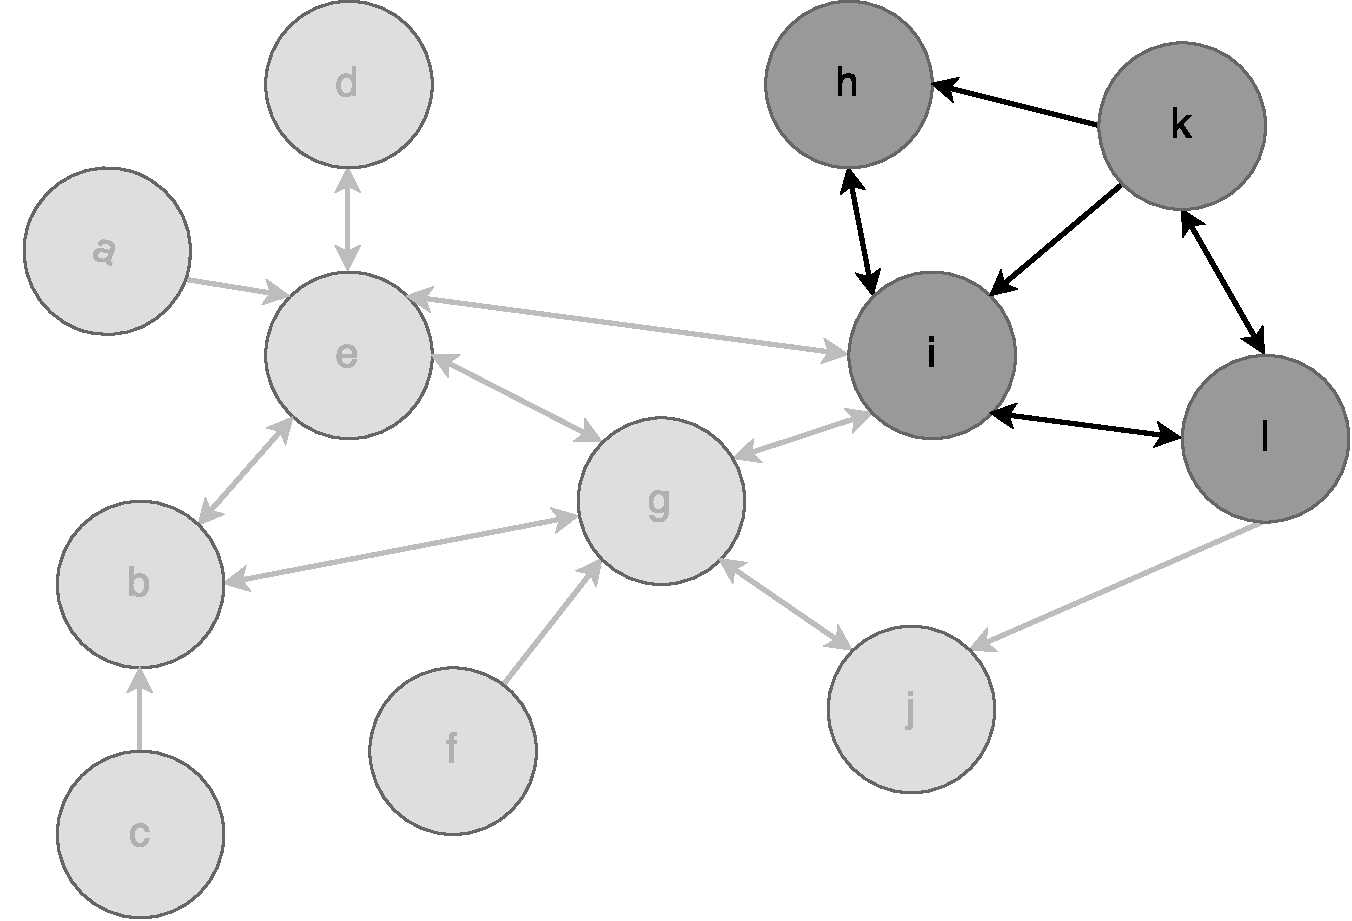
\includegraphics[scale=0.32]{graphics/directed_network_example_betweenness.pdf}
\end{figure}

\note{
L<-> is the edges going both ways\\
L is all outgoing edges
}
\end{frame}

\begin{frame}
\frametitle{Feature Selection}
The feature \textit{PageRank} measures centrality based on ingoing edges
\begin{columns}
\begin{column}{0.8\textwidth}\centering
	\begin{block}{\small PageRank}\centering
		$pr(g) = 1-d + d(\frac{pr(b)}{2}+\frac{pr(e)}{4} + \frac{pr(f)}{1} + \frac{pr(i)}{4} + \frac{pr(j)}{1})$
	\end{block}
\end{column}
\end{columns}
\begin{figure}
	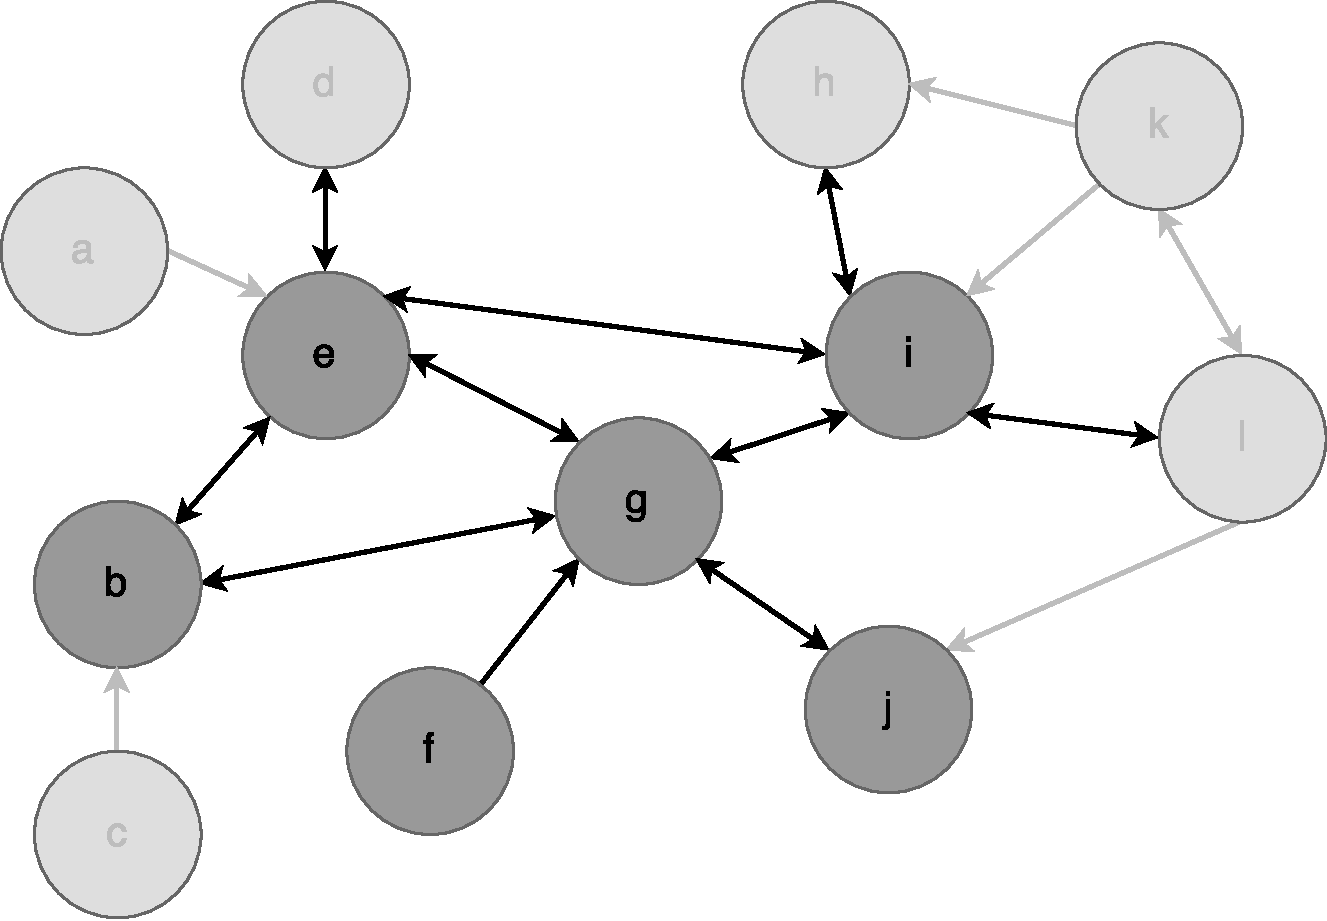
\includegraphics[scale=0.32]{graphics/directed_network_example_pagerank.pdf}
\end{figure}

\note{
L<-> is the edges going both ways\\
L is all outgoing edges
}
\end{frame}

\begin{frame}
\frametitle{Feature Selection}
\textit{Transitivity} measures is the local clustering coefficient which gives the probability of a vertexes neighbours being connected
\begin{columns}\centering
\begin{column}{0.8\textwidth}
	\begin{block}{\small Transitivity}\centering
		$C(v_i) = \frac{|\{e_{jk}\ :\  v_j,v_k\ \in\ N_i,\ e_{jk}\ \in\ E\}|}{k_i(k_i -1)}$
	\end{block}
\end{column}
\end{columns}
\begin{figure}
	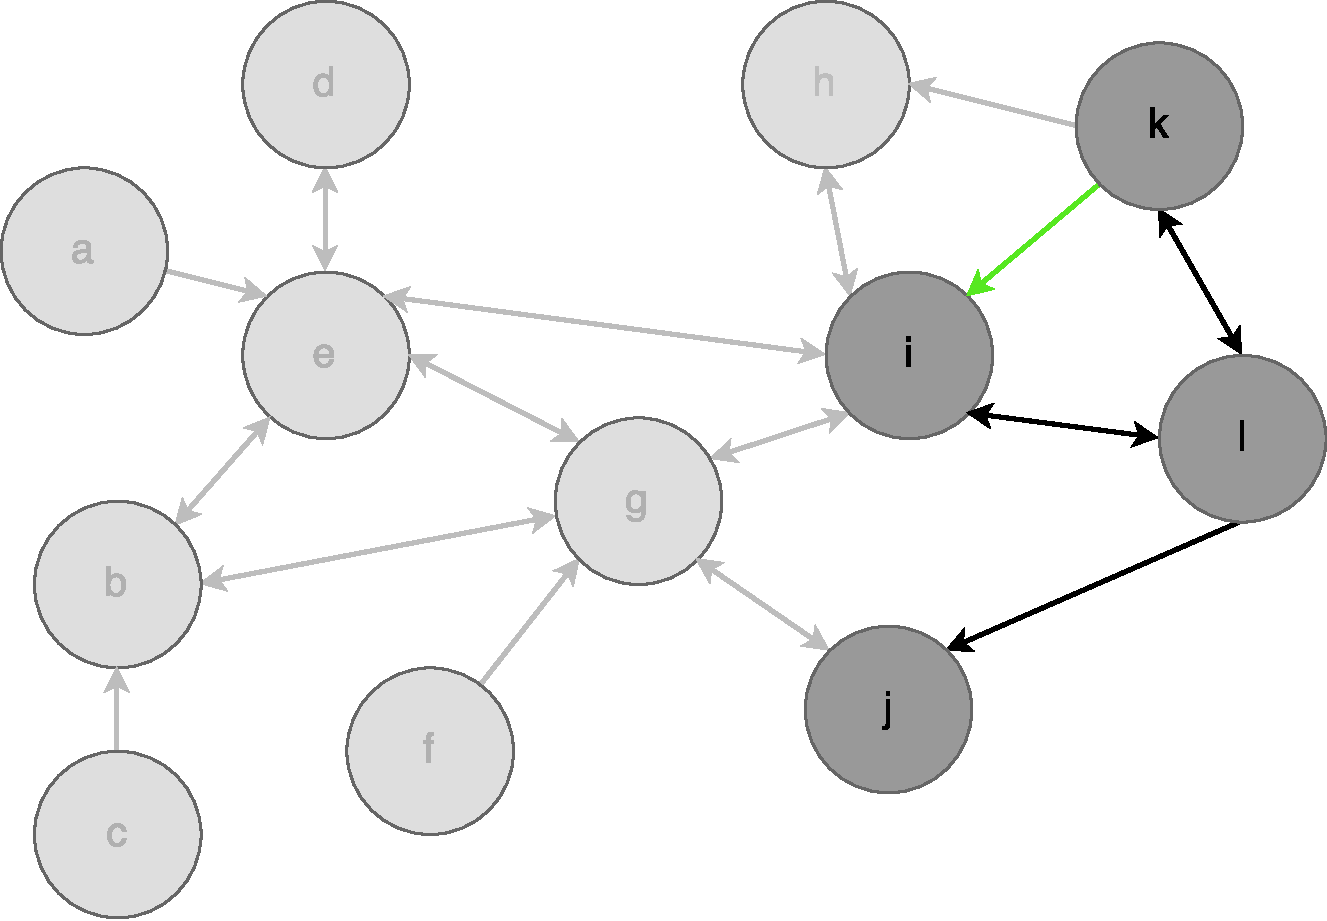
\includegraphics[scale=0.32]{graphics/directed_network_example_transitivity.pdf}
\end{figure}

\note{
L<-> is the edges going both ways\\
L is all outgoing edges
}
\end{frame}


\begin{frame}
\frametitle{Selected Features}
Summary of the features
\begin{itemize}
\item In-degree
\item Out-degree
\item Weighted in-degree
\item Weighted out-degree
\item Reciprocity 
\item New activity count
\item Social strategy
\item Betweenness centrality
\item PageRang
\item Transitivity
\end{itemize}

Features omitted from the walk-though 
\begin{itemize}
\item Weighted PageRank
\item Weighted transitivity
\end{itemize}
\end{frame}

\begin{frame}
\frametitle{Feature Extraction}

The result of feature extraction is a features $\times$ users feature matrix

\begin{figure}
	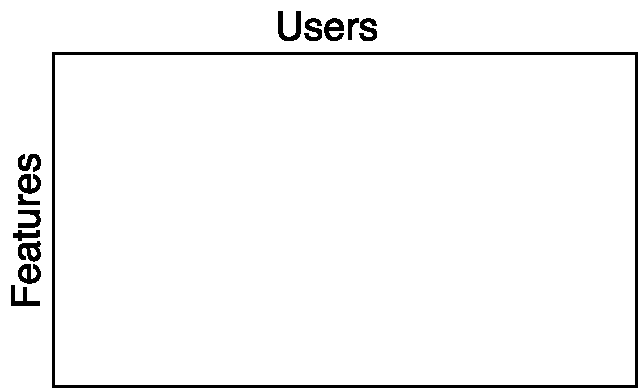
\includegraphics[scale=.5]{matrix}
\end{figure}

The features in the matrix is normalized by the use of feature scaling so that all values is within the interval of 1 and 0

\note{
Next is feature extraction\\
The authors do not argue for the selected features\\
12 was selected.
}
\end{frame}

\begin{frame}
\frametitle{Role Discovery}
\begin{columns}\centering
	\begin{column}{0.5\textwidth}
		\begin{block}{\small Non-negative Matrix Factorization}\centering
			$X \approx UV$
		\end{block}
		\end{column}
\end{columns}
\begin{figure}
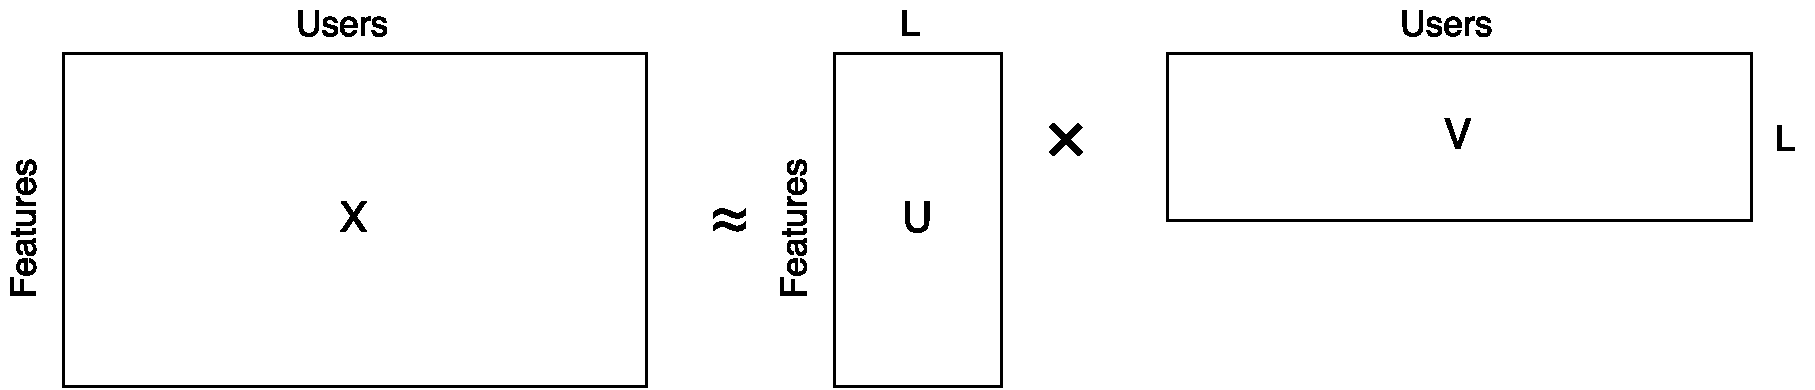
\includegraphics[scale=.3]{graphics/nmf}
\end{figure}

\begin{itemize}
\item Matrix U is role features 
\item Matrix V is membership weights for the roles for each user
\end{itemize}
\note{
\begin{itemize}
\item Frobenius NMF updated with euclidean distance
\item U and V are initialized with left and right matrix from nndsvd (Modified svd)

\end{itemize}
}
\end{frame}

\begin{frame}
\frametitle{Selection of L}
\begin{columns}
\begin{column}{0.5\textwidth}
\begin{block}{\small Root Mean Squired Error}\centering
$RMSE = \sqrt{\frac{1}{|X|} \sum\limits_{(u,f) \in X}(X_{u,f}-X'_{u,f})^2}$
\end{block}
\end{column}
\end{columns}
\begin{columns}
	\begin{column}{0.5\textwidth}
	\begin{figure}\caption{Facebook}
		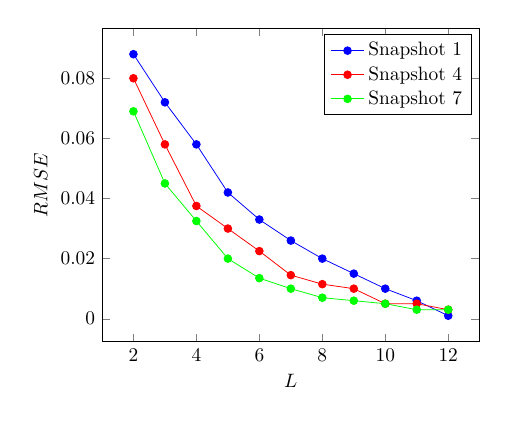
\begin{tikzpicture}[scale=0.7]
    \begin{axis}[
    	scaled ticks=false, 
    	tick label style={/pgf/number format/fixed},
        xlabel=$L$,
        ylabel=$RMSE$]
    \addplot[mark=*,blue] plot coordinates {
        (2, 0.088)
        (3, 0.072)
        (4, 0.058)
        (5, 0.042)
        (6, 0.033)
        (7, 0.026)
        (8, 0.020)
        (9, 0.015)
        (10, 0.010)
        (11, 0.006)
        (12, 0.001)
    };
    \addlegendentry{Snapshot 1}

    \addplot[color=red,mark=*]
        plot coordinates {
        (2, 0.08)
        (3, 0.058)
        (4, 0.0375)
        (5, 0.030)
        (6, 0.0225)
        (7, 0.0145)
        (8, 0.0115)
        (9, 0.01)
        (10, 0.005)
        (11, 0.005)
        (12, 0.003)
        };
    \addlegendentry{Snapshot 4}
    
    \addplot[color=green,mark=*]
        plot coordinates {
        (2, 0.069)
        (3, 0.045)
        (4, 0.0325)
        (5, 0.020)
        (6, 0.0135)
        (7, 0.010)
        (8, 0.007)
        (9, 0.006)
        (10, 0.005)
        (11, 0.003)
        (12, 0.003)
        };
    \addlegendentry{Snapshot 7}
    \end{axis}
\end{tikzpicture}	
\end{figure}
	\end{column}
	
	\begin{column}{0.5\textwidth}
	\begin{figure}\caption{Scratch}
		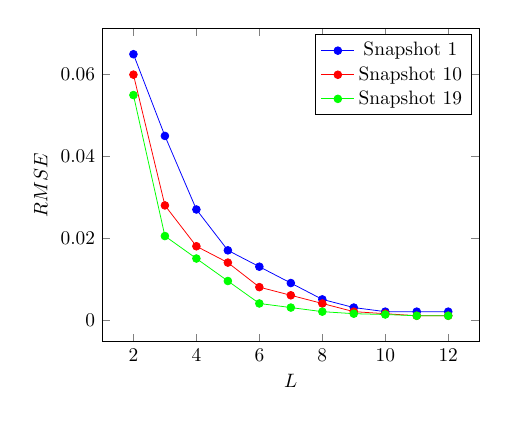
\begin{tikzpicture}[scale=0.7]
    \begin{axis}[
    	scaled ticks=false, 
    	tick label style={/pgf/number format/fixed},
        xlabel=$L$,
        ylabel=$RMSE$]
    \addplot[mark=*,blue] plot coordinates {
        (2, 0.065)
        (3, 0.045)
        (4, 0.027)
        (5, 0.017)
        (6, 0.013)
        (7, 0.009)
        (8, 0.005)
        (9, 0.003)
        (10, 0.002)
        (11, 0.002)
        (12, 0.002)
    };
    \addlegendentry{Snapshot 1}

    \addplot[color=red,mark=*]
        plot coordinates {
        (2, 0.06)
        (3, 0.028)
        (4, 0.018)
        (5, 0.014)
        (6, 0.008)
        (7, 0.006)
        (8, 0.004)
        (9, 0.002)
        (10, 0.0015)
        (11, 0.001)
        (12, 0.001)
    };
    \addlegendentry{Snapshot 10}
    
    \addplot[color=green,mark=*]
        plot coordinates {
        (2, 0.055)
        (3, 0.0205)
        (4, 0.015)
        (5, 0.0095)
        (6, 0.004)
        (7, 0.003)
        (8, 0.002)
        (9, 0.0015)
        (10, 0.0013)
        (11, 0.001)
        (12, 0.001)
        };
    \addlegendentry{Snapshot 19}
    \end{axis}
\end{tikzpicture}	
\end{figure}
	\end{column}
\end{columns}

\end{frame}

\begin{frame}
\frametitle{Tracing Roles}
\begin{columns}
\begin{column}{0.5\textwidth}
\begin{block}{\small Cosine Similarity}\centering
$sim(A_{i}, B_{i}) =\frac{\displaystyle\sum_{i=1}^n A_i B_i}{\sqrt{\displaystyle\sum_{i=1}^n A_{i}^2} \sqrt{\displaystyle\sum_{i=1}^n B_{i}^2}} $
\end{block}
\end{column}
\end{columns}

\begin{columns}
\begin{column}{0.5\textwidth}
Cosine similarity returns a value between -1 and 1
\begin{itemize}
\item -1 means that the vectors are opposites
\item 1 means they are exactly the same
\end{itemize} 
The article sets a threshold on 0.75 that roles from $S_t$ and $S_{t+1}$ must have similarity measure above
\end{column}
\begin{column}{0.25\textwidth}
\begin{figure}
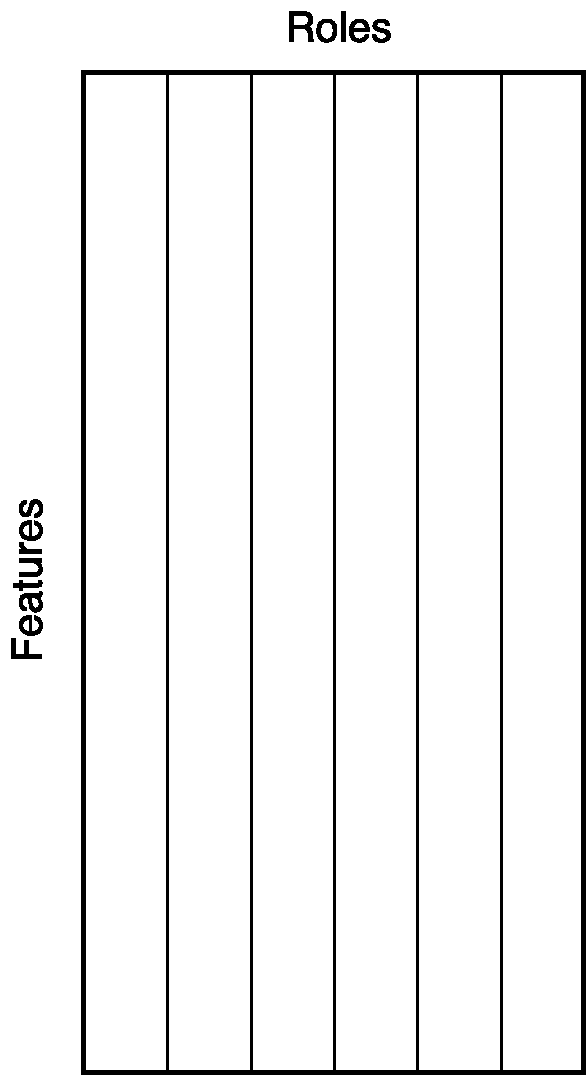
\includegraphics[scale=.2]{role_matrix}
\caption{$U_t$}
\end{figure}
\end{column}
\begin{column}{0.25\textwidth}
\begin{figure}
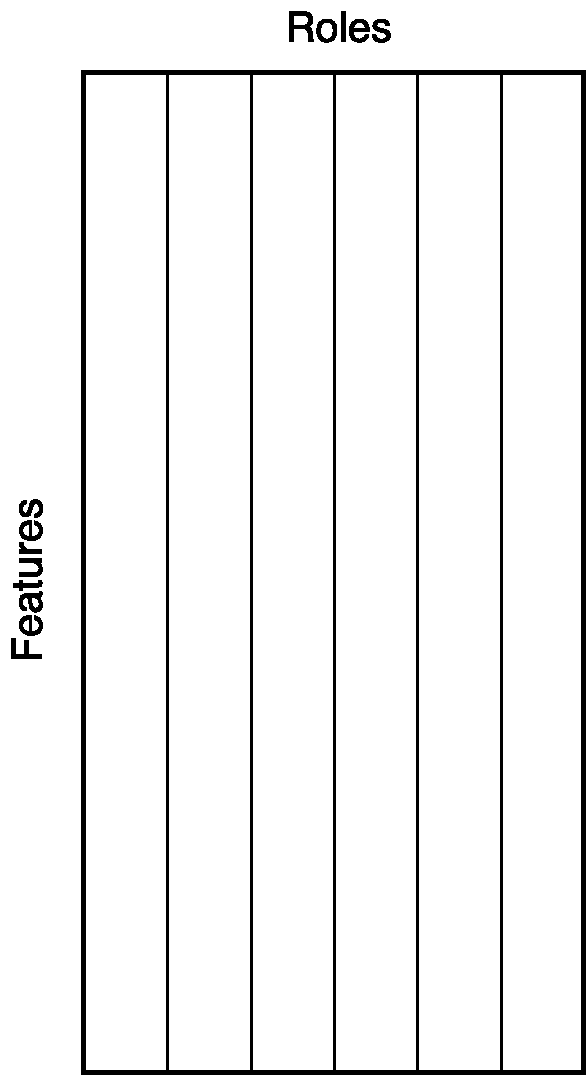
\includegraphics[scale=.2]{role_matrix}
\caption{$U_{t+1}$}
\end{figure}
\end{column}

\end{columns}
\end{frame}